%% =====================================================================
%% P5 (GT-Conditioned CVAE) 详细流程图 —— 独立可编译版本
%% 用法：pdflatex p5_flow_detailed.tex
%% 与 paper_P5/sections/method.tex 中的 fig:p5_flow 信息一致，
%% 但补充了各模块结构、维度与超参数标注。
%% =====================================================================
\documentclass[11pt]{article}
\usepackage[T1]{fontenc}
\usepackage{lmodern}
\usepackage{amssymb}
\usepackage{amsmath}
\usepackage{xcolor}
\usepackage[margin=0.4cm, paperwidth=26.5cm, paperheight=30cm]{geometry}
\usepackage{tikz}
\usetikzlibrary{positioning, fit, calc}

\pagestyle{empty}

\begin{document}
\thispagestyle{empty}
\centering
{\LARGE\bfseries P5 Algorithm: GT-Conditioned CVAE --- Detailed Flow}\\[2mm]
{\normalsize Training path (top) and deployment path (bottom); every
GT-consuming module is {\bfseries training-only}.}

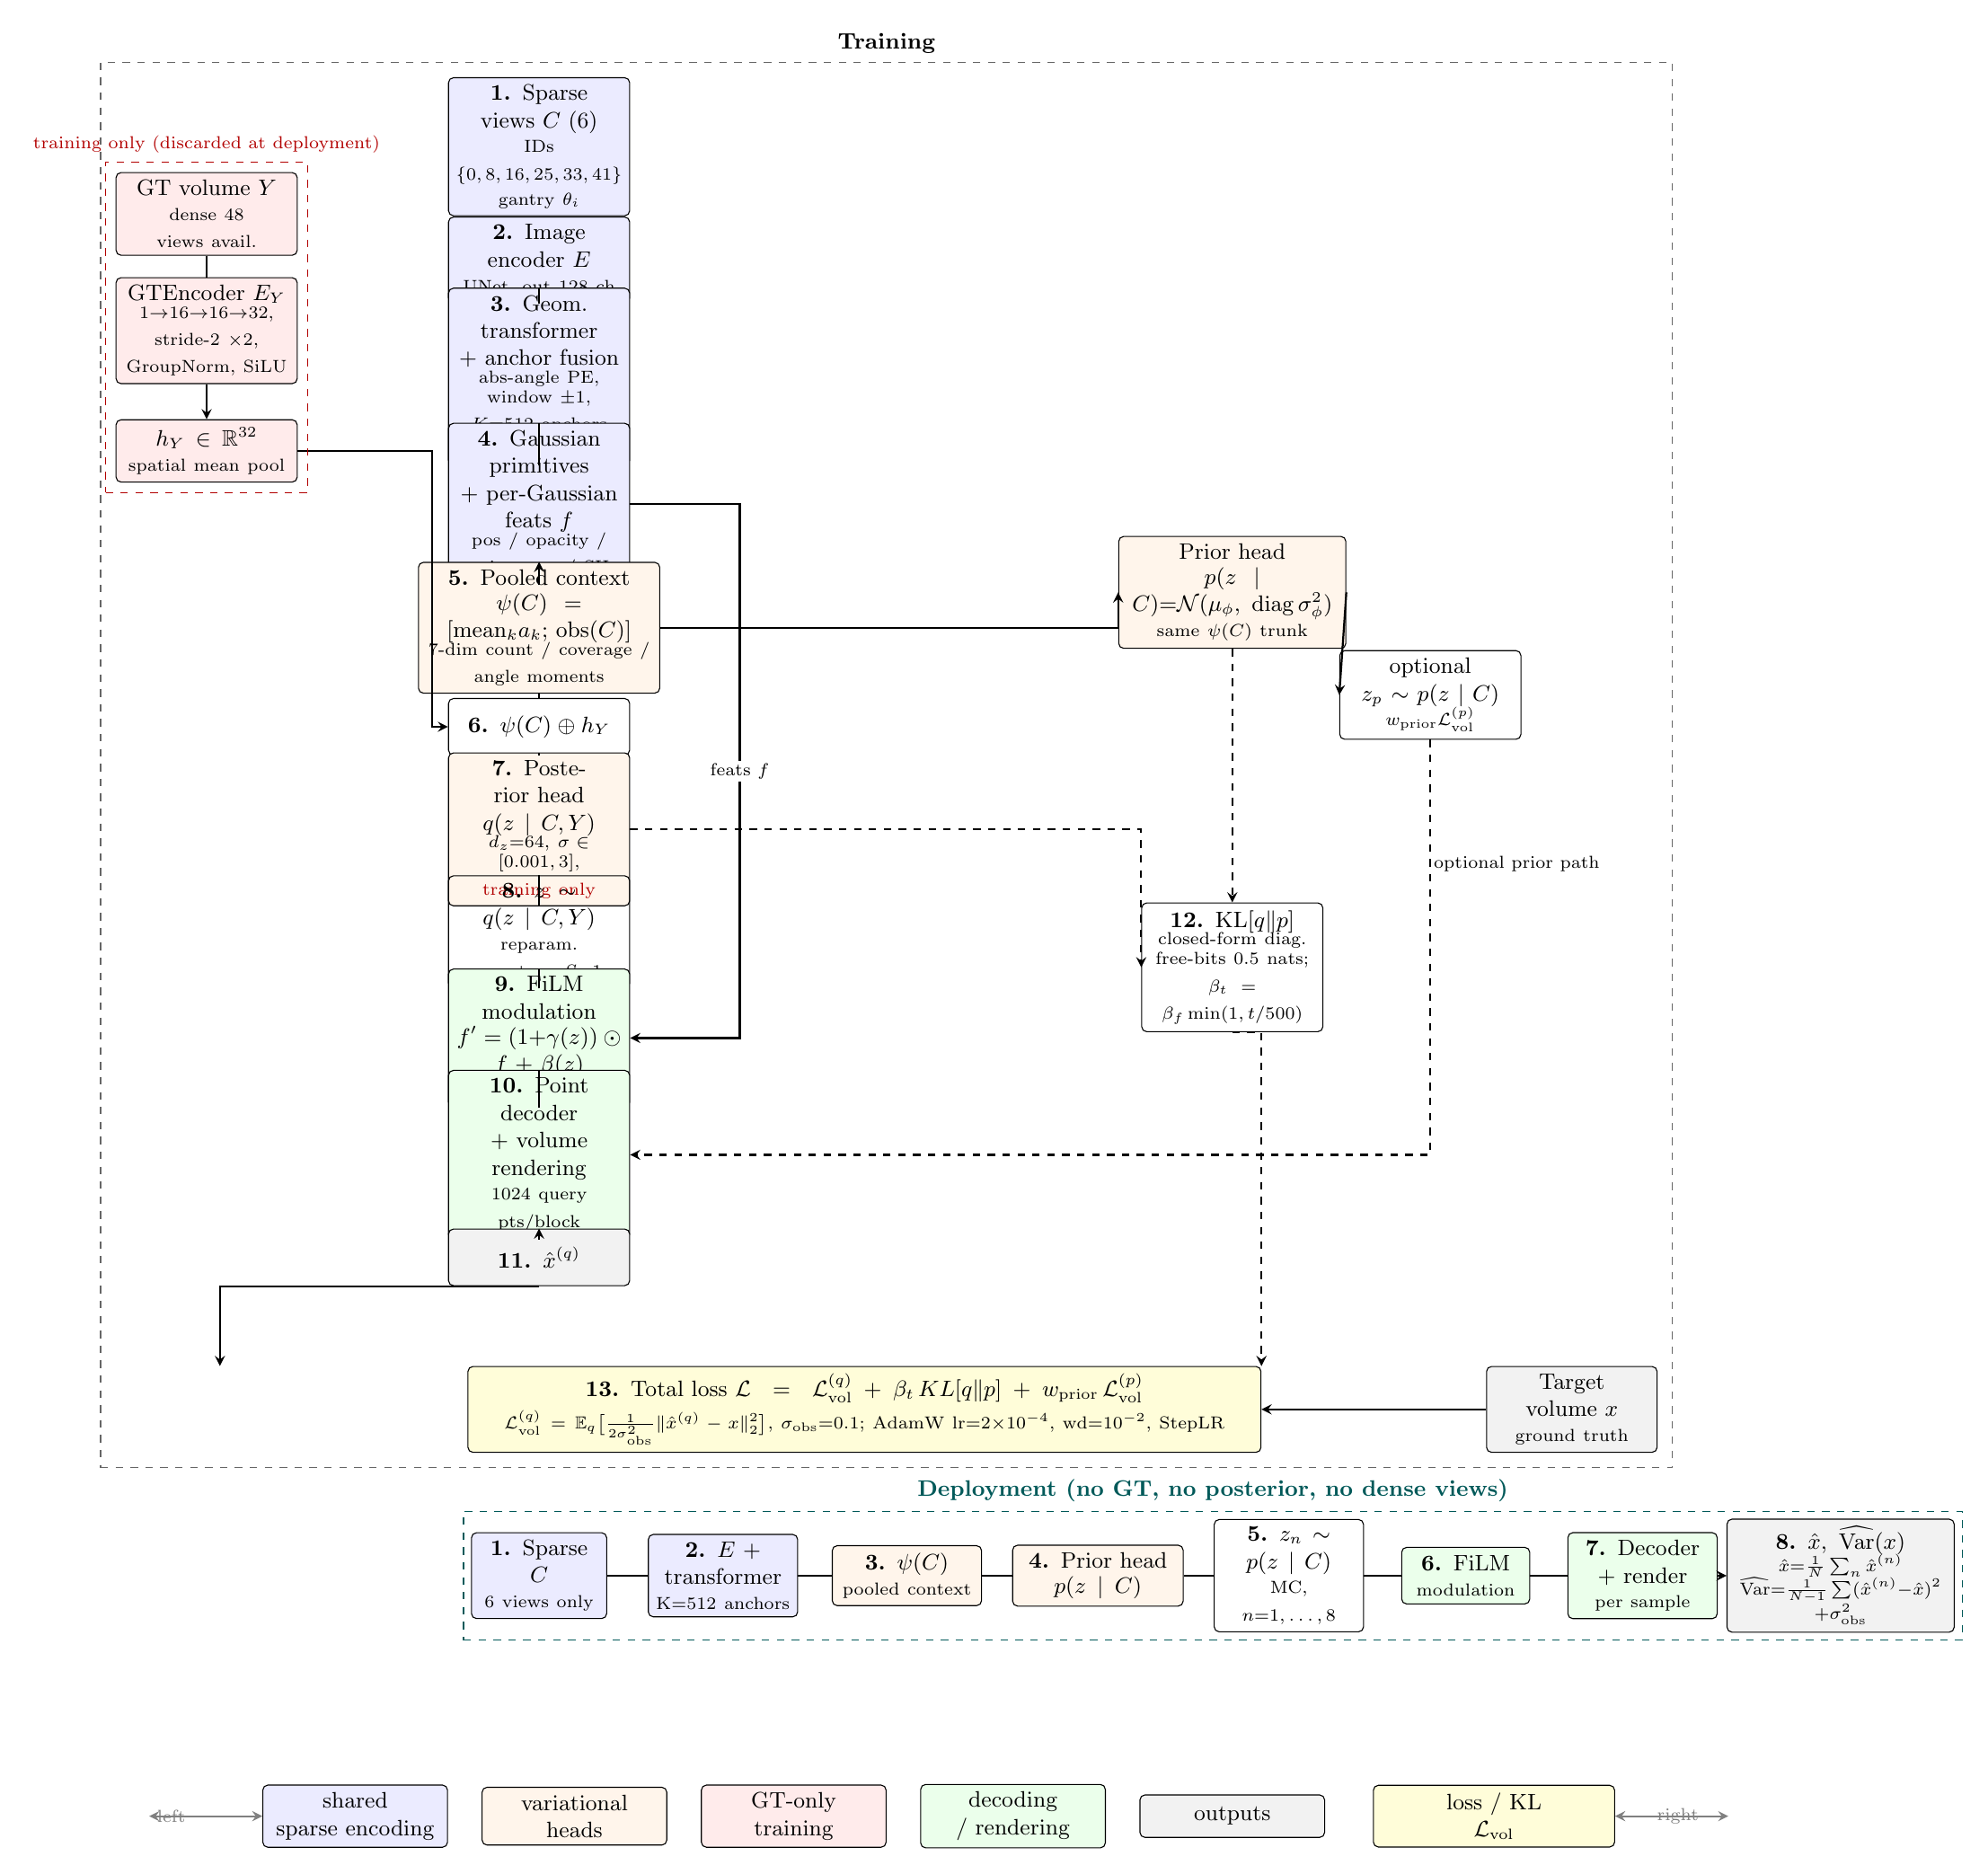
\begin{tikzpicture}[
    font=\small,
    >=stealth,
    box/.style={draw, rounded corners=2pt, align=center, inner sep=3pt,
                minimum height=8mm, text width=2.35cm},
    enc/.style={box, fill=blue!8},
    head/.style={box, fill=orange!8},
    gtenc/.style={box, fill=red!8},
    dec/.style={box, fill=green!8},
    outbox/.style={box, fill=gray!10},
    loss/.style={box, fill=yellow!15, text width=11cm},
    arr/.style={thick, ->},
    das/.style={thick, dashed, ->},
    lab/.style={font=\scriptsize, fill=white, inner sep=1pt},
]
% ---------------- 训练主列（稀疏上下文 → 后验采样 → 解码） ----------------
\node[enc]   (C)    at (0, 0)      {\textbf{1.} Sparse views $C$ (6)\\[-1pt]
    {\scriptsize IDs $\{0,8,16,25,33,41\}$}\\[-1pt]
    {\scriptsize gantry $\theta_i$}};
\node[enc]   (E)    at (0, -1.6)   {\textbf{2.} Image encoder $E$\\[-1pt]
    {\scriptsize UNet, out 128 ch}};
\node[enc]   (TF)   at (0, -3.25)  {\textbf{3.} Geom. transformer\\+ anchor fusion\\[-1pt]
    {\scriptsize abs-angle PE, window $\pm1$,\\$K{=}512$ anchors @ res 12}};
\node[enc]   (GS)   at (0, -5.05)  {\textbf{4.} Gaussian primitives\\+ per-Gaussian feats $f$\\[-1pt]
    {\scriptsize pos / opacity /\\aniso. cov / SH}};
\node[head, text width=3.2cm] (PSI)  at (0, -6.80)  {\textbf{5.} Pooled context\\[-1pt]
    $\psi(C)=[\mathrm{mean}_k a_k;\,\mathrm{obs}(C)]$\\[-1pt]
    {\scriptsize 7-dim count / coverage /\\angle moments}};
\node[box]   (CONC) at (0, -8.20)  {\textbf{6.} $\psi(C)\oplus h_Y$};
\node[head]  (Q)    at (0, -9.65)  {\textbf{7.} Posterior head\\$q(z\mid C,Y)$\\[-1pt]
    {\scriptsize $d_z{=}64$, $\sigma\!\in\![0.001,3]$,\\\color{red!70!black}training only}};
\node[box]   (ZQ)   at (0, -11.10) {\textbf{8.} $z\sim q(z\mid C,Y)$\\[-1pt]
    {\scriptsize reparam. $z{=}\mu{+}\sigma\varepsilon$, $S{=}1$}};
\node[dec]   (FILM) at (0, -12.60) {\textbf{9.} FiLM modulation\\[-1pt]
    $f'=(1{+}\gamma(z))\odot f+\beta(z)$\\[-1pt]
    {\scriptsize zero-init $\gamma{=}\beta{=}0$}};
\node[dec]   (DEC)  at (0, -14.25) {\textbf{10.} Point decoder\\+ volume rendering\\[-1pt]
    {\scriptsize 1024 query pts/block}};
\node[outbox](XQ)   at (0, -15.70) {\textbf{11.} $\hat{x}^{(q)}$};

% ---------------- GT 分支（仅训练，置于左侧） ----------------
\node[gtenc] (Y)    at (-4.7, -0.95) {GT volume $Y$\\[-1pt]
    {\scriptsize dense 48 views avail.}};
\node[gtenc] (GTE)  at (-4.7, -2.60) {GTEncoder $E_Y$\\[-1pt]
    {\scriptsize $1{\to}16{\to}16{\to}32$,\\stride-2 $\times2$, GroupNorm, SiLU}};
\node[gtenc] (hY)   at (-4.7, -4.30) {$h_Y\in\mathbb{R}^{32}$\\[-1pt]
    {\scriptsize spatial mean pool}};

% ---------------- 先验 / KL 分支（右侧） ----------------
\node[head, text width=3.0cm] (PriH) at (9.8, -6.30) {Prior head\\[-1pt]
    $p(z\mid C){=}\mathcal{N}(\mu_\phi,\;\mathrm{diag}\,\sigma_\phi^2)$\\[-1pt]
    {\scriptsize same $\psi(C)$ trunk}};
\node[box]   (PriZ) at (12.6, -7.75) {optional\\$z_p\sim p(z\mid C)$\\[-1pt]
    {\scriptsize $w_{\mathrm{prior}}\mathcal{L}_{\mathrm{vol}}^{(p)}$}};
\node[box]   (KL)   at (9.8, -11.60) {\textbf{12.} $\mathrm{KL}[q\|p]$\\[-1pt]
    {\scriptsize closed-form diag.\\free-bits 0.5 nats;\\$\beta_t=\beta_f\min(1,t/500)$}};

% ---------------- 损失与监督信号 ----------------
\node[loss]  (LOSS) at (4.6, -17.85) {\textbf{13.} Total loss
    $\mathcal{L}=\mathcal{L}_{\mathrm{vol}}^{(q)}+\beta_t\,KL[q\|p]
      +w_{\mathrm{prior}}\,\mathcal{L}_{\mathrm{vol}}^{(p)}$\\[2pt]
    {\scriptsize
    $\mathcal{L}_{\mathrm{vol}}^{(q)}=\mathbb{E}_{q}\big[\tfrac{1}{2\sigma_{\mathrm{obs}}^2}
    \|\hat{x}^{(q)}-x\|_2^2\big]$, $\sigma_{\mathrm{obs}}{=}0.1$;
    AdamW lr${=}2{\times}10^{-4}$, wd${=}10^{-2}$, StepLR}};
\node[outbox, text width=2.2cm] (TGT) at (14.6, -17.85) {Target volume $x$\\[-1pt]
    {\scriptsize ground truth}};

% ---------------- 训练箭头 ----------------
\draw[arr] (C) -- (E) -- (TF) -- (GS) -- (PSI);
\draw[arr] (GS.east) --++(1.55,0) |- (FILM.east)
    node[lab, pos=0.25] {feats $f$};
\draw[arr] (PSI) -- (CONC) -- (Q) -- (ZQ) -- (FILM) -- (DEC) -- (XQ);
\draw[arr] (Y) -- (GTE) -- (hY);
\draw[arr] (hY.east) --++(1.9,0) |- (CONC.west);
\draw[arr] (PSI.east) -| (PriH.west);
\draw[arr] (PriH.east) -- (PriZ.west);
\draw[das] (PriZ.south) |- (DEC.east)
    node[lab, pos=0.15, right] {optional prior path};
\draw[das] (Q.east) -| (KL.west);
\draw[das] (PriH.south) -- (KL.north);
\draw[das] (KL.south) -| (LOSS.north east);
\draw[arr] (XQ.south) -| ([xshift=-3.5cm]LOSS.north west);
\draw[arr] (TGT) -- (LOSS.east);

% ---------------- 训练/GT 标注框 ----------------
\node[draw=red!70!black, dashed, fit=(Y)(GTE)(hY), inner sep=4pt,
      label={[red!70!black, font=\scriptsize]above:training only (discarded at deployment)}] {};
\node[draw=black!60, dashed, fit=(C)(LOSS)(KL)(Y)(PriZ)(TGT), inner sep=6pt,
      label={[font=\small\bfseries]above:Training}] {};

% ---------------- 部署路径（水平） ----------------
\node[enc, text width=1.7cm]   (DC)    at (0.0, -20.2)  {\textbf{1.} Sparse $C$\\[-1pt]
    {\scriptsize 6 views only}};
\node[enc, text width=1.9cm]   (DE)    at (2.6, -20.2) {\textbf{2.} $E$ + transformer\\[-1pt]
    {\scriptsize K=512 anchors}};
\node[head, text width=1.9cm]  (DPSI)  at (5.2, -20.2) {\textbf{3.} $\psi(C)$\\[-1pt]
    {\scriptsize pooled context}};
\node[head, text width=2.2cm]  (DPRI)  at (7.9, -20.2) {\textbf{4.} Prior head\\[-1pt]
    $p(z\mid C)$};
\node[box, text width=1.9cm]   (DZ)    at (10.6, -20.2) {\textbf{5.} $z_n\sim p(z\mid C)$\\[-1pt]
    {\scriptsize MC, $n{=}1,\dots,8$}};
\node[dec, text width=1.6cm]   (DFILM) at (13.1, -20.2) {\textbf{6.} FiLM\\[-1pt]
    {\scriptsize modulation}};
\node[dec, text width=1.9cm]   (DDEC)  at (15.6, -20.2) {\textbf{7.} Decoder\\+ render\\[-1pt]
    {\scriptsize per sample}};
\node[outbox, text width=3.0cm](DX)    at (18.4, -20.2) {\textbf{8.} $\hat{x},\ \widehat{\mathrm{Var}}(x)$\\[-1pt]
    {\scriptsize $\hat{x}{=}\tfrac1N\sum_n\hat{x}^{(n)}$\\[-1pt]
    $\widehat{\mathrm{Var}}{=}\tfrac1{N{-}1}\sum(\hat{x}^{(n)}{-}\hat{x})^2$\\[-1pt]
    $+ \sigma_{\mathrm{obs}}^2$}};

\draw[arr] (DC) -- (DE) -- (DPSI) -- (DPRI) -- (DZ) -- (DFILM) -- (DDEC) -- (DX);

\node[draw=teal!70!black, dashed, fit=(DC)(DX), inner sep=3pt,
      label={[font=\small\bfseries, teal!70!black]above:Deployment (no GT, no posterior, no dense views)}] {};

% ---------------- 图例 ----------------
\node[enc, text width=2.4cm, minimum height=6mm]  (L1) at (-2.6, -23.6)  {shared\\sparse encoding};
\node[head, text width=2.4cm, minimum height=6mm] (L2) at (0.5, -23.6)   {variational\\heads};
\node[gtenc, text width=2.4cm, minimum height=6mm](L3) at (3.6, -23.6)   {GT-only\\training};
\node[dec, text width=2.4cm, minimum height=6mm]  (L4) at (6.7, -23.6)   {decoding\\/ rendering};
\node[outbox, text width=2.4cm, minimum height=6mm](L5) at (9.8, -23.6)  {outputs};
\node[loss, text width=3.2cm, minimum height=6mm] (L6) at (13.5, -23.6)  {loss / KL\\$\mathcal{L}_{\mathrm{vol}}$};

\draw[<->, thick, gray] (L1.west) --++(-1.6,0);
\draw[<->, thick, gray] (L6.east) --++(1.6,0);
\node[gray, font=\scriptsize] at (-2.6-1.6-1.0, -23.6) {left};
\node[gray, font=\scriptsize] at (13.5+1.6+1.0, -23.6) {right};
\end{tikzpicture}

\vspace{2mm}
{\scriptsize\itshape
Note: at deployment the GT encoder and the posterior head are never
instantiated; the decoder consumes sparse-view context features modulated by
$z\sim p(z\mid C)$ exactly as at training.}
\end{document}